\section{Profiling Results}
\label{sec:profiling}

\begin{figure}
\centering
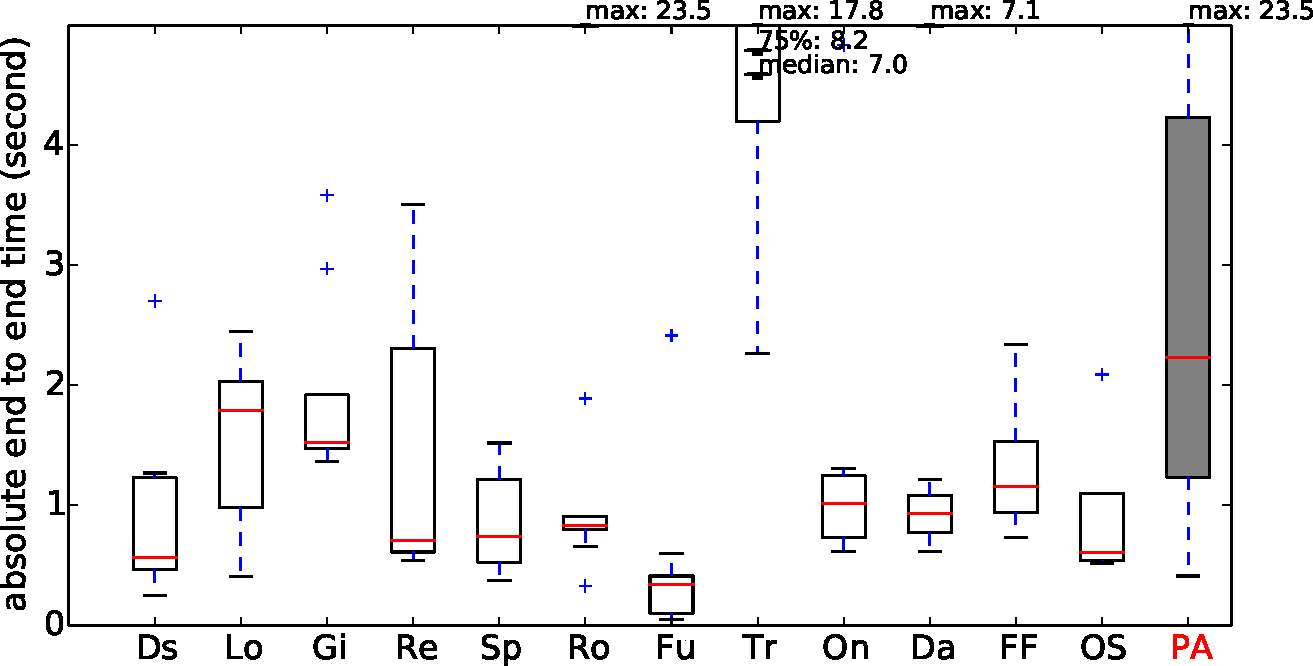
\includegraphics[height=1.75in, width=3.5in]{hownotto/EndToEnd}
\caption{End-to-end page loading time
}
\label{fig:eoeFig}
{\footnotesize Measured for top 10 time-consuming pages per application. Box: 25 to 75 percentile; Red line: median; PA: problematic actions from all 12 applications (see Section~\ref{sec:meth_profile}).\par}
\end{figure}


\begin{figure}
\centering
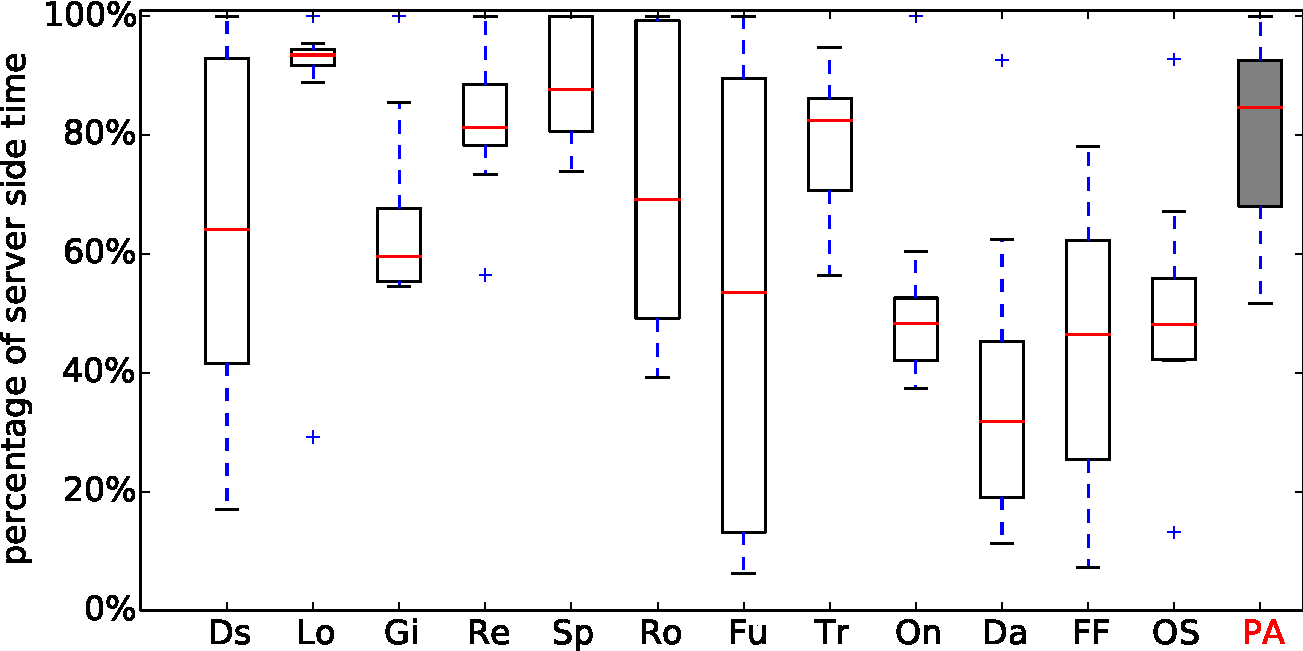
\includegraphics[height=1.75in, width=3in]{hownotto/Percentage}
\caption{Percentage of server time among end-to-end time}
{\footnotesize Measured for top 10 most time-consuming pages per application.
Red line: median; PA: problematic actions from all 12 applications (see Section~\ref{sec:meth_profile})}
\vspace{-0.2in}
\label{percentageFig}
\end{figure}

\begin{comment}
\begin{figure}
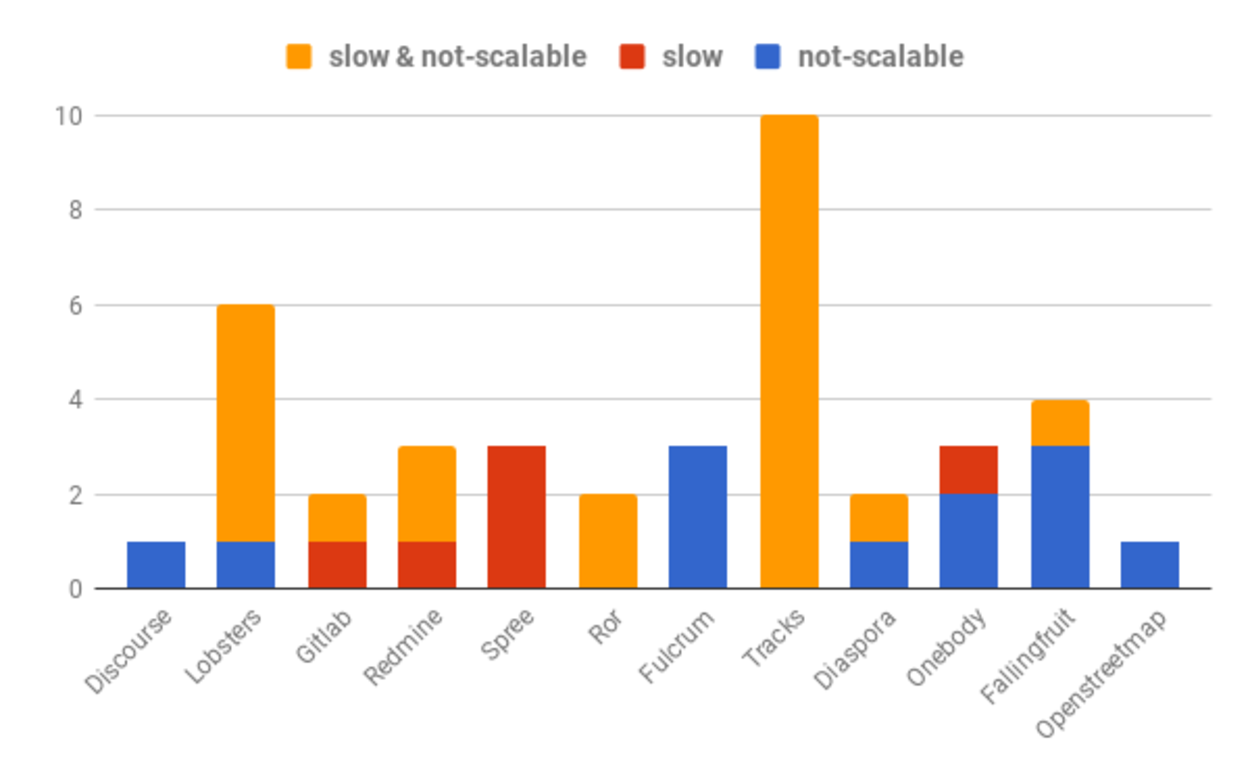
\includegraphics[height=2.2in, width=3.5in]{hownotto/probAct}
\caption{Number of problematic actions}
\label{probAct}
\end{figure}
\end{comment}
\paragraph{\bf{End-to-end loading time}} 
We identify the 10 pages with the most loading time for every application under the 20,000-record database configuration and plot their average end-to-end page loading time in
Figure~\ref{fig:eoeFig}. 11 out of 12 applications have pages whose average end-to-end loading time (i.e., from browser sending the URL request to page finishing loading) exceeds 2 seconds; 6 out of 12 applications have pages that take more than 3 seconds to load. \textit{Tracks} performs the worst: all of its top 10 most time-consuming pages take more than 2 seconds to load. 
%\shan{75\% of top 10 actions?} 
Note that, our workload is 
{\it smaller} or, for some applications, {\it much smaller} than today's real-world workload. Considering how the real-world workload's size will continue growing,
these results indicate that performance problems are prevalent and critical for deployed Rails applications.

\vspace{-0.08in} 
\paragraph{\bf{Server vs. client}}
We break down the end-to-end loading time of the top 10 pages in each 
application into server time (i.e., time for executing controller action, including view rendering and data access, on Rails server), 
client time (i.e., time for loading the DOM in the browser), and network time (i.e., time for data transfer between server and browser).  %\cong{We need to say what's the network latency. Maybe what browser client side uses also matters?} 
As shown in Figure~\ref{percentageFig}, server time contributes to at least 40\% of the end-to-end-latency for more than half of the top 10 pages in all but 1 application.\footnote{Part of the server time could overlap with the client time or the network time. However, our measurement shows that the overlap is negligible.}
Furthermore, over $50\%$ of problematic pages spend more than 80\% of the loading time on Rails server, as shown by the rightmost bar (labeled {\bf PA}) in Figure~\ref{percentageFig}.
%Furthermore, inefficiency in server computation could also affect network latency, as we will see later.
%Our profiling also indicates that server time scales much worse than client time xxx.
This result further motivates us to study the performance problems on the server side of ORM applications.
\vspace{-0.08in} 
\paragraph{\bf{Problematic server actions}}
Table~\ref{tab:probAct} shows the number of problematic actions for each application identified using
the methodology discussed in Section~\ref{sec:meth_profile}. In total, there are \numpactions problematic actions identified from the top 10 most time-consuming actions of every application. Among them, 34 have scalability problems and 28 take more than 1 second of server time. Half of the pages that correspond to these 40 problematic actions take more than 2 seconds to load, as shown in the rightmost bar (labeled {\bf PA}) in Figure~\ref{fig:eoeFig}.
In addition, we find 64 performance issues in these 40 problematic actions, and we will discuss them in detail in Section~\ref{sec:causes}.
%Server time contributes to more than half of the end-to-end time of all the problematic actions (right-most bar in Figure \ref{probAct}). \alvin{didn't we already discuss this in the last paragraph?} 
%\shan{how many have $>1$ second time?}\shan{Hmm, the figure seems to show much fewer number of actions with scalability problems}.

\begin{table}
\centering
\footnotesize
\caption{Number of problematic actions in each application}
\begin{tabular}{@{\hspace{0.1in}}l@{\hspace{0.1in}}l@{\hspace{0.1in}}l@{\hspace{0.1in}}l@{\hspace{0.1in}}l@{\hspace{0.1in}}l@{\hspace{0.1in}}l@{\hspace{0.1in}}l@{\hspace{0.1in}}l@{\hspace{0.1in}}l@{\hspace{0.1in}}l@{\hspace{0.1in}}l@{\hspace{0.1in}}l@{\hspace{0.1in}}}
\toprule
App & Ds & Lo & Gi & Re & Sp & Ro & Fu & Tr & Da & On & FF & OS  \\
\midrule
slow & 0 & 0 & 1 & 1 & 3 & 0 & 0 & 0 & 0 & 1 & 0 & 0 \\
not-scalable & 1 & 1 & 0 & 0 & 0 & 0 & 2 & 0 & 1 & 2 & 3 & 1 \\
slow \& not-scalable & 0 & 5 & 1 & 2 & 0 & 2 & 1 & 10 & 1 & 0 & 1 & 0\\
 \bottomrule
\end{tabular}
\label{tab:probAct}
\vspace{-0.25in}
\end{table}
